\section{Ansari-Bradley Test}
\subsection{Background}
\subsubsection{$\chi^2$ Distribution and $F$ Distribution}
The $\chi^2$ distribution is obtained directly from independent, standard normal random variables. Let $Z_i$, $i = 1,2, \dots, n$, be $n$ independent random variables, each distribution as standard normal. Define a new random variable as the sum of the squares of the $Z_i$:
\[X = \sum_{i=1}^{n}Z_i^2\]
Then, $X$ has what is known as a $\chi^2$ distribution with $n$ degree of freedom.

Another important distribution for statistics and econometrics is the $F$ distribution. In particular, the $F$ distribution will be used for testing hypotheses in the context of multiple regression analysis.

To define an $F$ random variable, Let $X_1 ~ \chi_{k_1}^2$ and $X_2 ~ \chi_{k_2}^2$ and assume that $X_1$ and $X_2$ are independent. Then the random variable
\[F = \frac{X_1 / k_1}{X_2 / k_2}\]
has an $F$ distribution with $(k_1, k_2)$ degree of freedom. We denote this as $F ~ F_{k_1, k_2}$.
\subsubsection{$F$-test of Equality of Variances}
In statistics, an $F$-test of equality of variances is a test for the null hypothesis that two normal populations have the same variance. 

\begin{itemize}
	\item Let $X_1, \dots, X_n$ and $Y_i, \dots, Y_n$ be iid samples from two populations which each has a normal distribution.
	\item The expected values for the two populations can be different.
	\item The Hypothesis is that the variances are equal.
\end{itemize}

Sample means are 
\[\bar{X} = \frac{1}{n} \sum_{i = 1}^{n} X_i, ~\bar{Y} = \frac{1}{m} \sum_{i=1}^{m}.\]

Sample variances are
\[S_X^2 = \frac{1}{n-1} \sum_{i=1}^{n}(X_i - \bar{X})^2, ~S_Y^2 = \frac{1}{m-1} \sum_{i=1}^{m}(Y_i - \bar{Y})^2.\]

Then the test statistic is an $F$-distribution with $n-1$ and $m-1$ degrees of freedom if the null hypothesis of equality of variacne is true.
\[F = \frac{S_X^2}{S_Y^2}\]

Otherwise it follows an $F$-distribution scaled by the ratio of true variances. The null hypothesis is rejected if $F$ is either too large or too small based on the desired alpha level 


\subsection{Assumption}
Ansari-Bradley Test is an non-parametric version of $F$-test. The null hypothesis of interest here is that the $X$ and $Y$ variable have the same probability distribution but their common distribution is not specified. 

We have the following assumptions for Ansari-Bradley Test:
\begin{itemize}
	\item $X_i$, $i \le m$, iid from continues population 1 with distribution $F$;
	\item $Y_j$, $j \le n$, iid from continues population 2 with distribution $G$;
	\item $X_i's$ and $Y_j's$ mutually independent;
	\item $F$ and $G$  have the same median $\theta$.
\end{itemize}
Note that $X_i$ and $Y_i$ are continues random variable. Also, Ansari-Bradley test works with different median between samples but here we assume two samples have the same median, $\theta$, for simplicity.

The alternative hypothesis can be that $Y$ population has the same general form as the $X$ population, but they could have different scales. It can be written as 
\[\frac{X - \theta}{\eta_x} \stackrel{d}{=} \frac{Y - \theta}{\eta_y}\]

, where $\stackrel{d}{=}$ means ``has the same distribution'', $\eta_x$ and $\eta_y$ are the scale parameters of $F$ and $G$, respectively.

The parameter of interest is the ratio of the scale parameters, $\gamma = \frac{\eta_x}{\eta_y}$.

In terms of this location-scale parameter model with equal location parameters, the null hypothesis is 
\[H_0: \gamma^2 = 1\]
, corresponding to the assertion that the population scale parameters are equal.

why $\gamma^2$ instead of $\gamma$. Sometimes we cannot calculate the variance (second moment), e.g. Poisson Distribution, during  standardization, so we keep the squaring later after the standardization.
\subsection{Hypothesis Test}

\begin{itemize}
	\item $H_0: \gamma^2 = 1$
	\item $H_1: \gamma^2 > 1$ (right-tailed test)
	\item $H_1: \gamma^2 < 1$ (left-tailed test)
	\item $H_1: \gamma^2 \neq 1$ (two-sided test)
\end{itemize}

\subsubsection{Assign Scores}
Order the combined samples of $N = m + n$ $X_i's$ and $Y_j$'s from least to greatest.
\begin{itemize}
	\item Assign the score 1 to both the smallest and the largest observations in this combined sample.
	\item Assign the score 2 to the 2nd smallest and 2nd largest.
	\item ...
\end{itemize}
In the end, we will get a list of score such that
\begin{itemize}
	\item If $N$ is an even integer, the array of assigned scores is 
	\[1, 2, \dots, \frac{N}{2}, \frac{N}{2}, \dots, 2, 1\]
	\item If $N$ is an odd integer, the array of assigned score is 
	\[1, 2, \dots, \frac{N-1}{2},\frac{N+1}{2},\frac{N-1}{2}, \dots, 2, 1\]
\end{itemize}
\subsubsection{Two-sample Scale Statistic}
Let $R_j$ be the score assigned to $Y_j$, $j = 1, \dots, n$.
The test statistic is $C = \sum_{j=1}^{n} R_j$.

Under the null hypothesis, we have
\[\E C = \frac{n(N+2)}{4}, \Var C = \frac{mn(N+2)}{48(N-1)}\]

The big idea is that we calculate the critical value $c_\alpha$ based on the Type I error of the experiment design and decide whether to reject the null hypothesis by comparing $C$ and $c_\alpha$. Intuitively, \textbf{if $\gamma^2 > 1$}, the $X$ values would tend to be more spread out than the $Y$ values. Thus, the $Y_j's$ would tend to get larger scores than the $X_i's$. \textbf{Then $C$ would tend to be larger}.

Note that $\gamma$ shows in the hypothesis to describe the data but the test statistics is actually $C$, the sum of ranks in $Y$.

The p-value of the hypothesis test can be calculated from the build-in R function \texttt{ansari.test}.

\begin{center}
	\lstinputlisting[language=R, caption=Ansari Example]{code/ansari.R}
\end{center}

\begin{figure}[H]
	\centering
	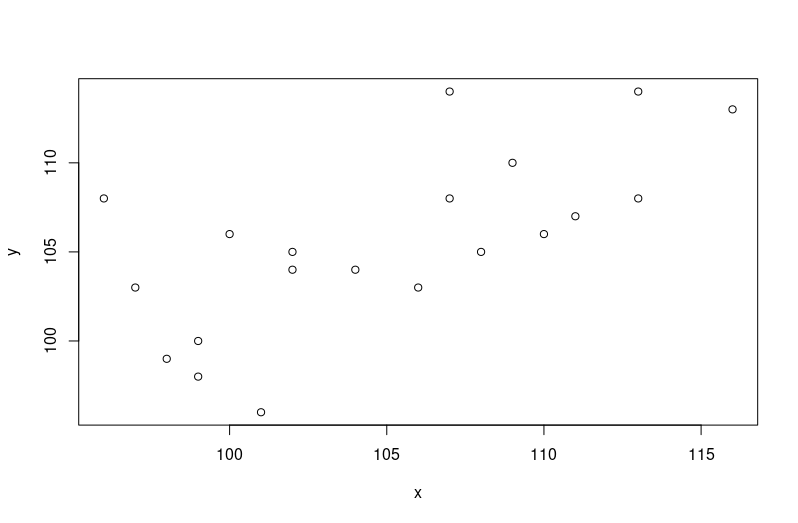
\includegraphics[width=0.7\linewidth]{fig/ansari}
	\caption{}
	\label{fig:ansari}
\end{figure}

Note that the range of X and Y are very similar, which indicates that they share the same dispersion. Also, in the Ansari-Bradley test, we get p-val = 0.1815, so that we cannot reject the null hypothesis.

